\section{Discussion}
\subsection{Why LFP wins in this model}
Three mechanisms act together. First, LFP's higher round-trip efficiency cuts charging energy by \gridratio\%. Second, ageing at 30--34$^\circ$C is far slower per cycle for lithium, so one LFP pack outlasts about seven lead-acid packs. Third, fewer replacements mean fewer manufactured packs and less lead entering the recycling chain. The lead-acid life (\lifeLA{} months) is close to the 8--12 months reported in the field \citep{fe2024}, so the baseline is realistic; the LFP life of \lifeLFP{} months rests on laboratory-derived ageing laws and a cycle-life range, and has not been observed in Bangladeshi service, which is why operator data remain the most valuable next step. The ranking agrees with LCA findings that LFP is preferable where many daily cycles occur \citep{jasper2025,yudhistira2022}.

\subsection{Temperature: what matters and what does not}
Regional temperature does \emph{not} separate Khulna, Chuadanga and Rajshahi: mean battery temperatures differ by \Tspread$^\circ$C and every ranking is identical. Chemistry choice is therefore robust to site within the south-west. The temperature effect operates through the seasonal cycle, heat waves, and above all the battery's temperature rise above ambient (\cref{tab:scen}), the largest single uncertainty. Measuring pack temperature in service is a higher priority than adding weather stations.

\subsection{Carbon: a smaller prize than health, but robust}
A full switch saves about \fleetLFPa{}~Mt\,CO$_2$e per year at 1.4~M bikes, and the saving holds across manufacturing footprints of 50--110~kg\,CO$_2$e/kWh and grid factors of 0.55--0.70. As the grid decarbonises the operational saving falls while the embodied saving remains. The carbon case alone is not the strongest argument for switching; cost and lead are stronger.

\subsection{Lead, workers and public health}
Used lead-acid batteries are collected, broken open, and their lead plates smelted, often by hand and close to homes and farmland. Pure Earth describes informal recycling that contaminates and poisons workers and nearby residents \citep{pureearth_smep}; ESDO identifies it as a primary contributor to lead-pollution hotspots \citep{esdo2021}. The IEDCR bulletin reports that about 36~million children (60\%) are poisoned by lead, and that market screening in Dhaka, Rajshahi, Khulna and Barishal found 24\% of 197 consumer samples above reference lead levels; home assessments in 47 Khulna households found high lead in metal and ceramic cookware and toys \citep{das2026}. Children are most vulnerable: the World Health Organization notes that no safe level of lead exposure is known \citep{who_lead}. Remediation helps but only partly: soil lead fell 96\% at an abandoned Savar site while child blood lead fell 35\% \citep{chowdhury2021}; the IEDCR bulletin reports a 20\% fall at Mirzapur, where hotspot soil dropped from about 100{,}000 ppm to 60--100 ppm \citep{das2026}; and a Tangail study reports 22\% \citep{eos2026}. The fact that blood lead falls much less than soil lead suggests other sources persist, so removing the source of new contamination is as important as cleaning old sites. Between 70\% and 80\% of ULAB recycling is reported to be informal \citep{dailystar80,pureearth_smep,cpd2025}, and e-rickshaws and easy-bikes generate about 77\% of ULABs \citep{unep_ulab}.

Our model supplies the \emph{quantity} side: by extending battery life from about 12 to about 84~months, an LFP conversion removes \leadLow--\leadHigh{}~kt of lead per year from the recycling stream at 1.4~M bikes. It does not estimate how much of that lead would reach people; that needs emission and exposure data that do not yet exist, and other sources (paint, spices, cookware) also contribute. \begin{figure}[t]\centering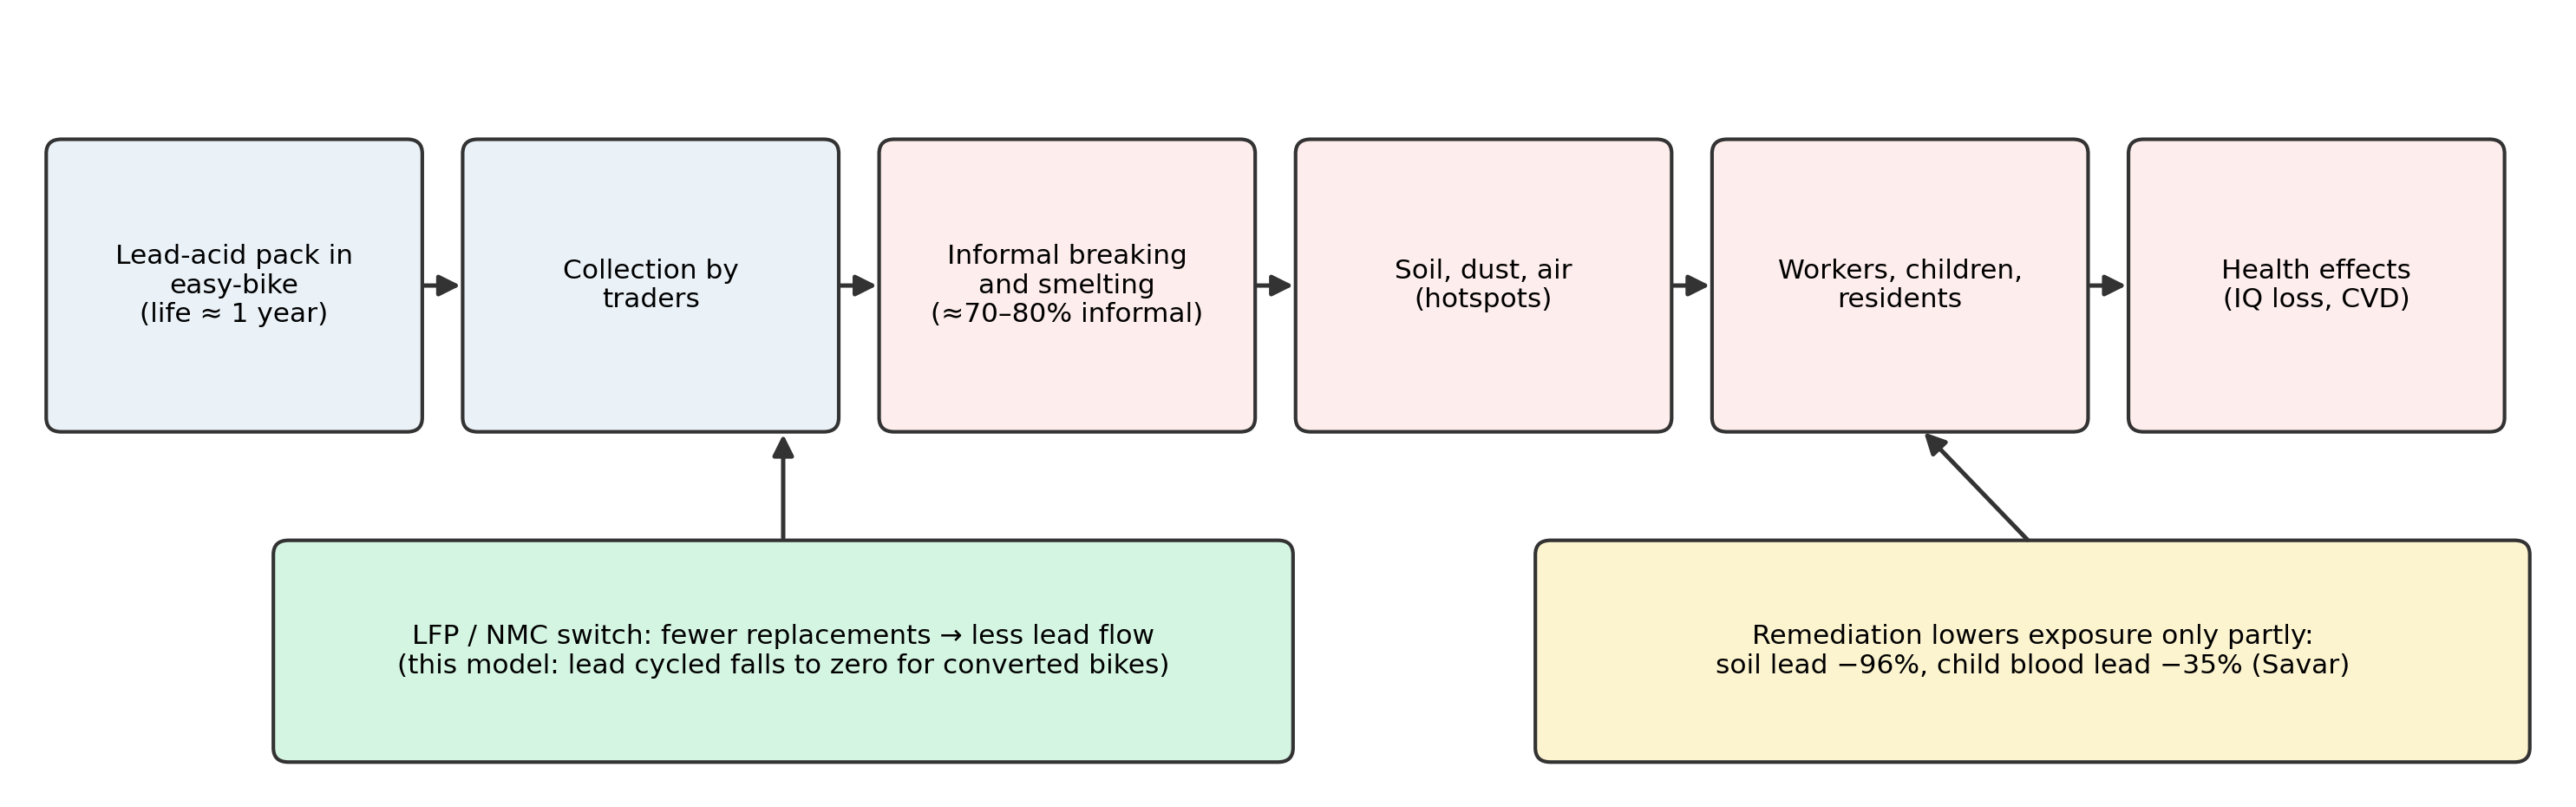
\includegraphics[width=\textwidth]{fig_lead.png}\caption{Pathway from lead-acid easy-bike batteries to exposure (schematic) and the point where an LFP switch acts; remediation figures from \citep{chowdhury2021}.}\label{fig:lead}\end{figure}

\subsection{Policy implications}
(i)~\emph{Up-front finance}: the BDT \premium{} premium is repaid in about \paybackYr{} year, so the barrier is capital access, not total cost; pay-as-you-go and battery-swap schemes address this \citep{smep2024}. (ii)~\emph{Taxes and duties}: current taxes on lithium batteries are described as unfavourable \citep{smep2024}, while the break-even price of about BDT \beLFP{} leaves large room for relief. (iii)~\emph{ULAB regulation}: the 2021 Hazardous Waste (e-waste) Management Rules reportedly cover household but not e-rickshaw lead batteries \citep{smep2024}. (iv)~\emph{Lithium end-of-life}: a collection and recycling route must exist before volumes grow.

\subsection{Limitations}\label{sec:limits}
\begin{itemize}[nosep]
\item \textbf{No operator records.} Battery temperature rise, operating days and scrap value are scenarios; daily distance is calibrated to a published energy per charge. The model is plausible against published ranges but not validated against operator data.
\item \textbf{Cycle-limited life.} Calendar ageing is not modelled; the LFP life of \lifeLFP{} months (about 7 years) may be optimistic in hot, rough service, though the 10-year cost includes only one replacement.
\item \textbf{Vendor-level capacity curves} for the temperature dependence of capacity; the effect is small between 20 and 45$^\circ$C.
\item \textbf{Monthly temperature.} Hourly data would capture daily peaks and charging-time heat.
\item \textbf{Single-site field study.} Duty inputs come from one instrumented bike and a survey in Gopalganj and Khulna \citep{chowdhury2026}.
\item \textbf{Fleet size.} 1.4~M and 3--4~M are both reported; results scale linearly.
\item \textbf{Weight, fire safety and imports} are not modelled.
\item \textbf{Lead flow is not exposure.}
\item \textbf{Tariff.} The BDT 11.36/kWh rate is from the June 2026 order as reported by the press; wholesale prices were revised again in August 2026 \citep{observer2026}. Tariffs of 7.70--16.24 change the cost gap by less than 3\% (\cref{tab:scen}).
\end{itemize}
